%% fig_convolutions.tex   (generated by make_round32.py; do not edit by hand)
%% The excess of the steps of a cycle of pieces (prop:nothingenters), and the one path whose products can act on the diagonal at n = 3 (thm:esixdiagonal).
\documentclass[tikz,border=8pt]{standalone}
\usepackage{amsmath,amssymb}
\usetikzlibrary{arrows.meta,calc,decorations.pathreplacing}
%% palette.tex -- shared colour definitions for the figures
\definecolor{PInk}{RGB}{26,32,44}
\definecolor{PBlue}{RGB}{37,82,139}
\definecolor{PTeal}{RGB}{23,127,125}
\definecolor{POchre}{RGB}{193,138,44}
\definecolor{PClay}{RGB}{178,74,58}
\definecolor{PSlate}{RGB}{108,122,137}
\definecolor{PViolet}{RGB}{110,86,150}
\definecolor{WBlue}{RGB}{223,234,246}
\definecolor{WTeal}{RGB}{220,238,236}
\definecolor{WOchre}{RGB}{250,240,218}
\definecolor{WClay}{RGB}{247,229,224}
\definecolor{WSlate}{RGB}{238,241,244}
\definecolor{PMag}{RGB}{158,58,110}
\definecolor{PGrass}{RGB}{62,124,66}
\definecolor{PAmber}{RGB}{214,112,38}
\definecolor{PIndigo}{RGB}{58,64,140}
\definecolor{PRule}{RGB}{176,186,197}

%% shared macros so the standalone figures match the paper
\providecommand{\QQ}{\mathbb{Q}}
\providecommand{\ZZ}{\mathbb{Z}}
\providecommand{\RR}{\mathbb{R}}
\providecommand{\CC}{\mathbb{C}}
\providecommand{\PP}{\mathbb{P}}
\providecommand{\Kx}{K^{\times}}
\providecommand{\HW}{W}
\providecommand{\Nm}{\mathrm{N}}
\providecommand{\Hdg}{\mathrm{Hdg}}
\providecommand{\NS}{\mathrm{NS}}
\providecommand{\cA}{\mathcal{A}}
\providecommand{\cD}{\mathcal{D}}
\providecommand{\cF}{\mathcal{F}}
\providecommand{\cP}{\mathcal{P}}
\providecommand{\cO}{\mathcal{O}}
\providecommand{\cQ}{\mathcal{Q}}
\providecommand{\bbar}[1]{\overline{#1}}
\providecommand{\ch}{\operatorname{ch}}
\providecommand{\End}{\mathrm{End}}
\providecommand{\Ext}{\operatorname{Ext}}
\providecommand{\Supp}{\operatorname{Supp}}

\begin{document}
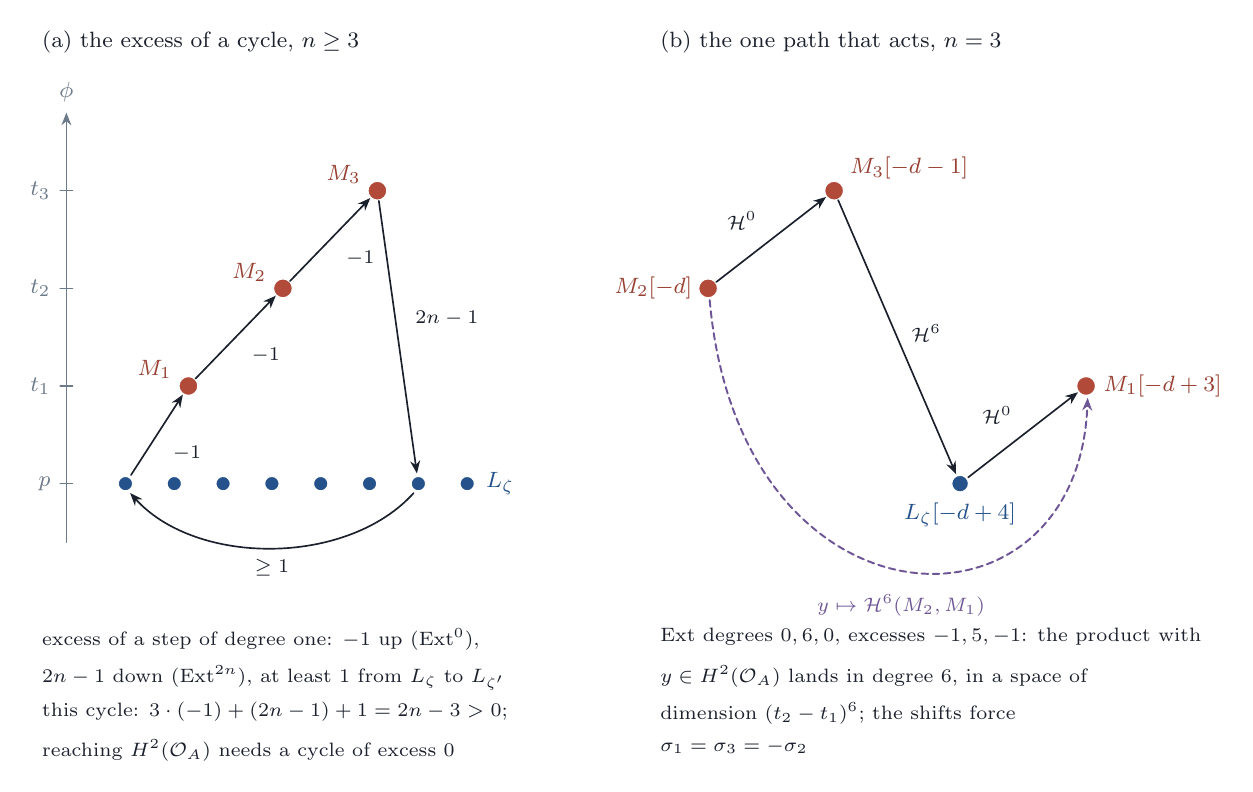
\begin{tikzpicture}[x=1cm,y=1cm,line join=round,line cap=round,
  font=\small,text=PInk,lbl/.style={inner sep=1pt}]
  \draw[PSlate,line width=0.5pt,-{Stealth[length=4.6pt,width=3.6pt]}] (0.0000,-0.7440) -- (0.0000,4.7120);
  \draw[PSlate,line width=0.45pt] (-0.0800,0.0000) -- (0.0800,0.0000);
  \draw[PSlate,line width=0.45pt] (-0.0800,1.2400) -- (0.0800,1.2400);
  \draw[PSlate,line width=0.45pt] (-0.0800,2.4800) -- (0.0800,2.4800);
  \draw[PSlate,line width=0.45pt] (-0.0800,3.7200) -- (0.0800,3.7200);
  \path[fill=PBlue,draw=white,line width=0.40pt] (0.7500,0.0000) circle (2.60pt);
  \path[fill=PBlue,draw=white,line width=0.40pt] (1.3700,0.0000) circle (2.60pt);
  \path[fill=PBlue,draw=white,line width=0.40pt] (1.9900,0.0000) circle (2.60pt);
  \path[fill=PBlue,draw=white,line width=0.40pt] (2.6100,0.0000) circle (2.60pt);
  \path[fill=PBlue,draw=white,line width=0.40pt] (3.2300,0.0000) circle (2.60pt);
  \path[fill=PBlue,draw=white,line width=0.40pt] (3.8500,0.0000) circle (2.60pt);
  \path[fill=PBlue,draw=white,line width=0.40pt] (4.4700,0.0000) circle (2.60pt);
  \path[fill=PBlue,draw=white,line width=0.40pt] (5.0900,0.0000) circle (2.60pt);
  \path[fill=PClay,draw=white,line width=0.40pt] (1.5500,1.2400) circle (3.40pt);
  \path[fill=PClay,draw=white,line width=0.40pt] (2.7500,2.4800) circle (3.40pt);
  \path[fill=PClay,draw=white,line width=0.40pt] (3.9500,3.7200) circle (3.40pt);
  \draw[PInk,line width=0.6pt,-{Stealth[length=4.6pt,width=3.6pt]}] (0.8205,0.1092) -- (1.4795,1.1308);
  \draw[PInk,line width=0.6pt,-{Stealth[length=4.6pt,width=3.6pt]}] (1.6404,1.3334) -- (2.6596,2.3866);
  \draw[PInk,line width=0.6pt,-{Stealth[length=4.6pt,width=3.6pt]}] (2.8404,2.5734) -- (3.8596,3.6266);
  \draw[PInk,line width=0.6pt,-{Stealth[length=4.6pt,width=3.6pt]}] (3.9680,3.5913) -- (4.4520,0.1287);
  \draw[PInk,line width=0.6pt,-{Stealth[length=4.6pt,width=3.6pt]}] (4.4100,-0.1200) .. controls (3.5700,-1.0500) and (1.6500,-1.0500) .. (0.8100,-0.1200);
  \path[fill=PClay,draw=white,line width=0.40pt] (8.1500,2.4800) circle (3.40pt);
  \path[fill=PClay,draw=white,line width=0.40pt] (9.7500,3.7200) circle (3.40pt);
  \path[fill=PBlue,draw=white,line width=0.40pt] (11.3500,0.0000) circle (3.00pt);
  \path[fill=PClay,draw=white,line width=0.40pt] (12.9500,1.2400) circle (3.40pt);
  \draw[PInk,line width=0.6pt,-{Stealth[length=4.6pt,width=3.6pt]}] (8.2528,2.5596) -- (9.6472,3.6404);
  \draw[PInk,line width=0.6pt,-{Stealth[length=4.6pt,width=3.6pt]}] (9.8014,3.6006) -- (11.2986,0.1194);
  \draw[PInk,line width=0.6pt,-{Stealth[length=4.6pt,width=3.6pt]}] (11.4528,0.0796) -- (12.8472,1.1604);
  \draw[PViolet,line width=0.7pt,dash pattern=on 2.4pt off 1.6pt,-{Stealth[length=4.6pt,width=3.6pt]}] (8.1700,2.3300) .. controls (8.5500,-1.9840) and (12.8500,-2.1080) .. (12.9700,1.0900);
  \node[lbl,anchor=south,text=PSlate,font=\footnotesize] at (0.0000,4.8120) {$\phi$};
  \node[lbl,anchor=east,text=PSlate,font=\footnotesize] at (-0.1600,0.0000) {$p$};
  \node[lbl,anchor=east,text=PSlate,font=\footnotesize] at (-0.1600,1.2400) {$t_{1}$};
  \node[lbl,anchor=east,text=PSlate,font=\footnotesize] at (-0.1600,2.4800) {$t_{2}$};
  \node[lbl,anchor=east,text=PSlate,font=\footnotesize] at (-0.1600,3.7200) {$t_{3}$};
  \node[lbl,anchor=west,text=PBlue,font=\footnotesize] at (5.2900,0.0000) {$L_{\zeta}$};
  \node[lbl,anchor=east,text=PClay!85!black,font=\footnotesize] at (1.3800,1.4478) {$M_{1}$};
  \node[lbl,anchor=east,text=PClay!85!black,font=\footnotesize] at (2.5800,2.6878) {$M_{2}$};
  \node[lbl,anchor=east,text=PClay!85!black,font=\footnotesize] at (3.7800,3.9278) {$M_{3}$};
  \node[lbl,anchor=west,text=PInk,font=\scriptsize] at (1.3100,0.3839) {$-1$};
  \node[lbl,anchor=west,text=PInk,font=\scriptsize] at (2.3100,1.6239) {$-1$};
  \node[lbl,anchor=west,text=PInk,font=\scriptsize] at (3.5100,2.8639) {$-1$};
  \node[lbl,anchor=west,text=PInk,font=\scriptsize] at (4.3900,2.0961) {$2n-1$};
  \node[lbl,anchor=north,text=PInk,font=\scriptsize] at (2.6100,-0.9200) {$\ge1$};
  \node[lbl,anchor=west,text=PInk,font=\scriptsize] at (-0.3500,-1.9766) {excess of a step of degree one: $-1$ up ($\Ext^{0}$),};
  \node[lbl,anchor=west,text=PInk,font=\scriptsize] at (-0.3500,-2.4652) {$2n-1$ down ($\Ext^{2n}$), at least $1$ from $L_{\zeta}$ to $L_{\zeta'}$};
  \node[lbl,anchor=west,text=PInk,font=\scriptsize] at (-0.3500,-2.8992) {this cycle: $3\cdot(-1)+(2n-1)+1=2n-3>0$;};
  \node[lbl,anchor=west,text=PInk,font=\scriptsize] at (-0.3500,-3.3866) {reaching $H^{2}(\cO_{A})$ needs a cycle of excess $0$};
  \node[lbl,anchor=west,text=PInk,font=\footnotesize] at (-0.3500,5.6148) {(a) the excess of a cycle, $n\ge3$};
  \node[lbl,anchor=east,text=PClay!85!black,font=\footnotesize] at (7.9900,2.4800) {$M_{2}[-d]$};
  \node[lbl,anchor=west,text=PClay!85!black,font=\footnotesize] at (9.9100,4.0028) {$M_{3}[-d-1]$};
  \node[lbl,anchor=north,text=PBlue,font=\footnotesize] at (11.3500,-0.2000) {$L_{\zeta}[-d+4]$};
  \node[lbl,anchor=west,text=PClay!85!black,font=\footnotesize] at (13.1300,1.2400) {$M_{1}[-d+3]$};
  \node[lbl,anchor=east,text=PInk,font=\scriptsize] at (8.8100,3.3400) {$\mathcal{H}^{0}$};
  \node[lbl,anchor=west,text=PInk,font=\scriptsize] at (10.6900,1.9100) {$\mathcal{H}^{6}$};
  \node[lbl,anchor=east,text=PInk,font=\scriptsize] at (12.0500,0.8718) {$\mathcal{H}^{0}$};
  \node[lbl,anchor=north,text=PViolet,font=\scriptsize] at (10.6000,-1.3640) {$y\mapsto\mathcal{H}^{6}(M_{2},M_{1})$};
  \node[lbl,anchor=west,text=PInk,font=\scriptsize] at (7.5000,-1.9455) {$\Ext$ degrees $0,6,0$, excesses $-1,5,-1$: the product with};
  \node[lbl,anchor=west,text=PInk,font=\scriptsize] at (7.5000,-2.4466) {$y\in H^{2}(\cO_{A})$ lands in degree $6$, in a space of};
  \node[lbl,anchor=west,text=PInk,font=\scriptsize] at (7.5000,-2.9166) {dimension $(t_{2}-t_{1})^{6}$; the shifts force};
  \node[lbl,anchor=west,text=PInk,font=\scriptsize] at (7.5000,-3.3399) {$\sigma_{1}=\sigma_{3}=-\sigma_{2}$};
  \node[lbl,anchor=west,text=PInk,font=\footnotesize] at (7.5000,5.6148) {(b) the one path that acts, $n=3$};
\end{tikzpicture}
\end{document}
